\subsection{Data Models}
The data used in the land use model system can be described as an
integrated Data Model.   We describe in this section the data model 
used by SAM, and the data model proposed for AZ-SMART, focusing on
the first phase of the project.

\subsubsection{SAM Data Model}

The model presented in Figure \ref{figSAMDataModel} is developed from the
data documentation of SAM-IM.  The key tables in the current SAM system are the 
exlu, plan, and developments attribute tables and contents tables (which have 
a many to one relationship with the attribute tables to allow mixed use
representation).  There are no direct primary key - foreign key relationships that 
allow a database join among these three attribute tables.  Instead, they are spatially 
cross-referenced by the conversion to grids.  The various geographies used in SAM 
and their relationships are included in the top part of the E-R diagram, including 
census blocks, block groups, tracts, taz, raz, mpa, county, and state geographies.

\begin{figure}[h]
\begin{center}
%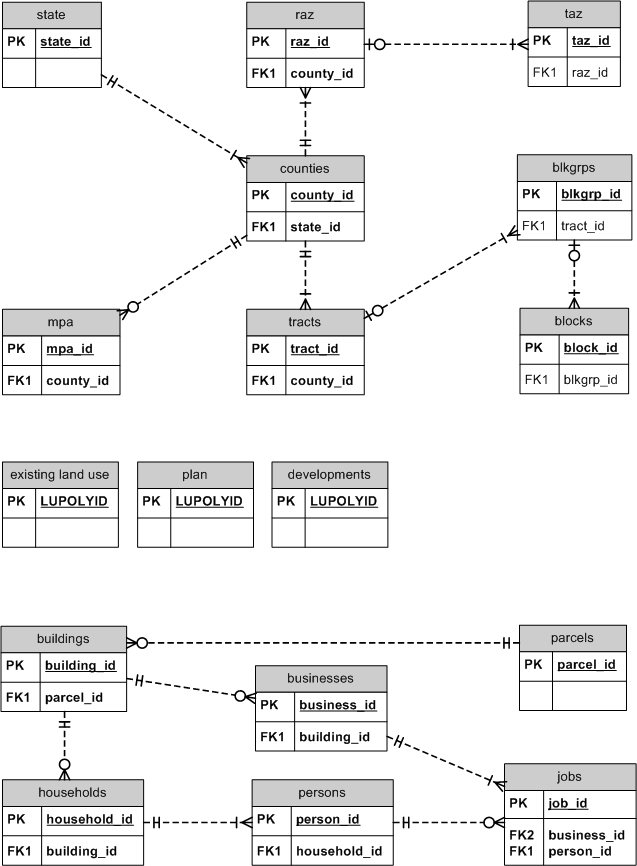
\includegraphics[scale=0.5]{figures/AZ-SMART_data_model_diagram.png}
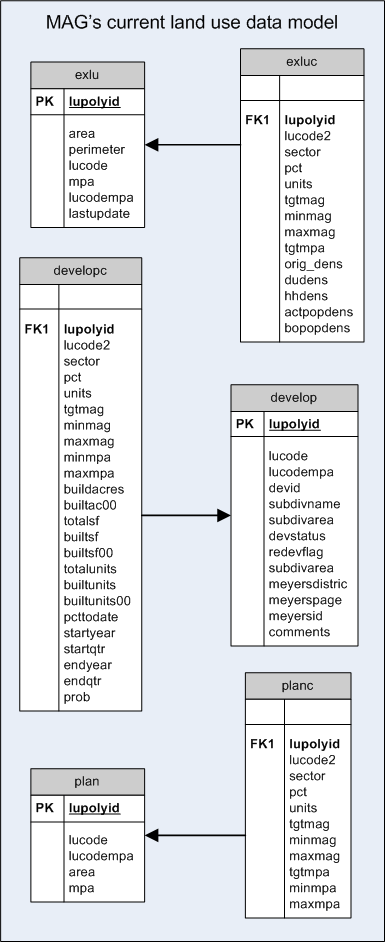
\includegraphics[scale=0.4]{../../datamodel/SAM-IM_data_model_diagram.png}
\caption{SAM-IM Data Model}
\label{figSAMDataModel}
\end{center}
\end{figure}


\subsubsection{AZ-SMART Data Model Using Land Use Polygons}

The model presented in Figure \ref{figLUPolyDataModel} presents the proposed data model for
the AZ-SMART project, focusing on an initial phase 1 implementation, making maximum use of
existing data.  It uses existing land use, planned developments, and land use plans just as
does the SAM model.  There are some major differences from the SAM data model, however.
First, we propose to handle buildings explicitly in the data model.  In the initial implementation, 
these buildings would be
imputed from the existing data, based on the land use and density of the existing land use
content records.  Land use polygons would contain attributes for
geographic ids for higher level features such as taz, raz, mpa, city, and county,
and other attributes such as land area, and attributes to be used in the scoring functions, which
we will refer to as the development probability functions.

We propose to use the \emph{Development Site} as a data object that initially would be equivalent to a
land use polygon, but would allow the data to also reflect a collection of land use polygons 
into one development site.  This will be particularly valuable when we move to parcels rather 
than land use polygons.  Development sites will have comprehensive plan assignments, so
it is possible to interpret for each development site what development restrictions apply to it.

The comprehensive plan is linked to a set of \emph{Development Constraints}, which indicate the types
and densities of development that are allowed to be developed on a particular Development Site.
The constraints are assumed not to apply to any Scheduled Developments that are provided
by the user as known events.  If a plan type is mixed use, then the constraint would be configured
to reflect this by a mixture of buildings and densities that would be permissible for development.

\emph{Development Templates} reflect prototypical kinds of
building development, with their associated land area.  We propose using a broad set of building
types, drawing on the SAM classification initially, and using the FAR and Units per Acre density
measures as a means of differentiating among different intensities of development within a building
type.  These templates can be created by examining recent development projects and creating a 
set of templates that would cover the range of projects being built or potentially under consideration. 
Development Constraints can be interpreted in terms of which Development Templates would be permitted
for development on each Development Site, based on the Plan Type, and other locational characteristics
of the site.   To represent mixe-use development, we structure the Development Template as having one
or more \emph{Building Components}, which characterize a building of a particular type and density.

\emph{Development Proposals} are Development Templates that can be considered for a specific
Development Site.  These are the Development Templates that are permitted by the Development
Constraints, and that fit within the land area of the Development Site.  The land area and other attributes
of the site may be drawn from the land use polygon(s) that comprise the Development Site.

Both Scheduled Developments and Development Proposals have a start year, a number of years to 
be fully developed, and a reference to a \emph{Development Velocity Function}.  These velocity
functions can be stored in a separate table for lookup.

Jobs and Households each are represented by their own tables, with one record per job and one per
 household.  Jobs have an id and a sector, and are assigned to a building record, which indicates that
they are on a particular land use polygon and in a particular type of building.  Households have
any needed socio-demographic characteristics and also are assigned to a building, which is 
itself assigned to a land use polygon.  Control totals for population and employment are each
represented in a table, with year, sector and employment for the employment control totals, and RAZ
to accommodate control totals specified at this level of geography (this could be modified as needed).
Similarly, population control totals would be specified year, RAZ and type.  These control totals could be
from previous runs of the mid-level model, or produced by interfacing to the model.

Flexible aggregation of data to TAZ, RAZ, City, County, and gridcell would be accommodated by this 
data model.  For most of these geographies, the data could be directly aggregated using the foreign
key relationships in the data model.  For gridcell representation, anything linked to the land use polygon
could be assigned to gridcells via a land use polygon to gridcell mapping table that contains the
fractional allocation of each land use polygon across the gridcells it overlaps with.  This mechanism
could also be used to query spatially and assign results to the land use polygon, building, job or household.

\begin{sidewaysfigure}[h]
\begin{center}
%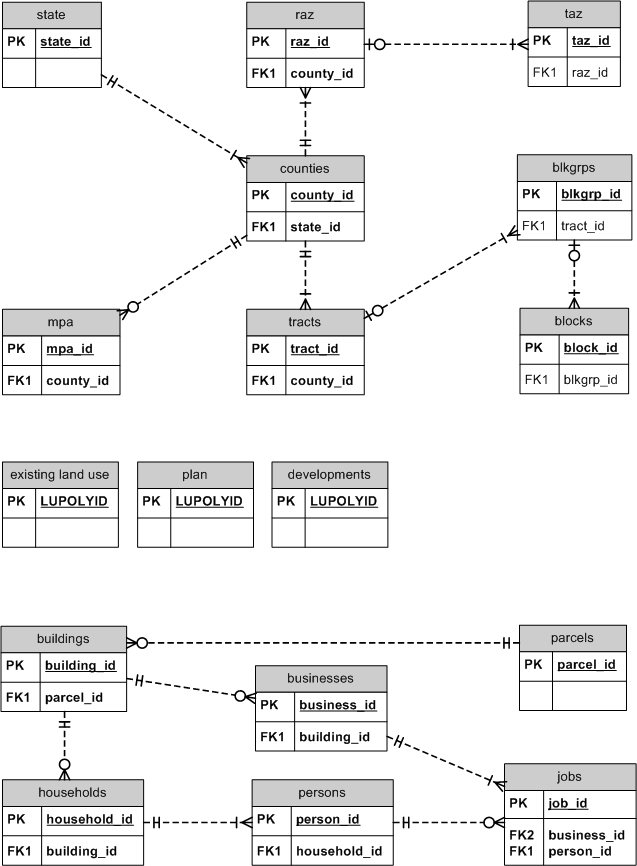
\includegraphics[scale=0.5]{figures/AZ-SMART_data_model_diagram.png}
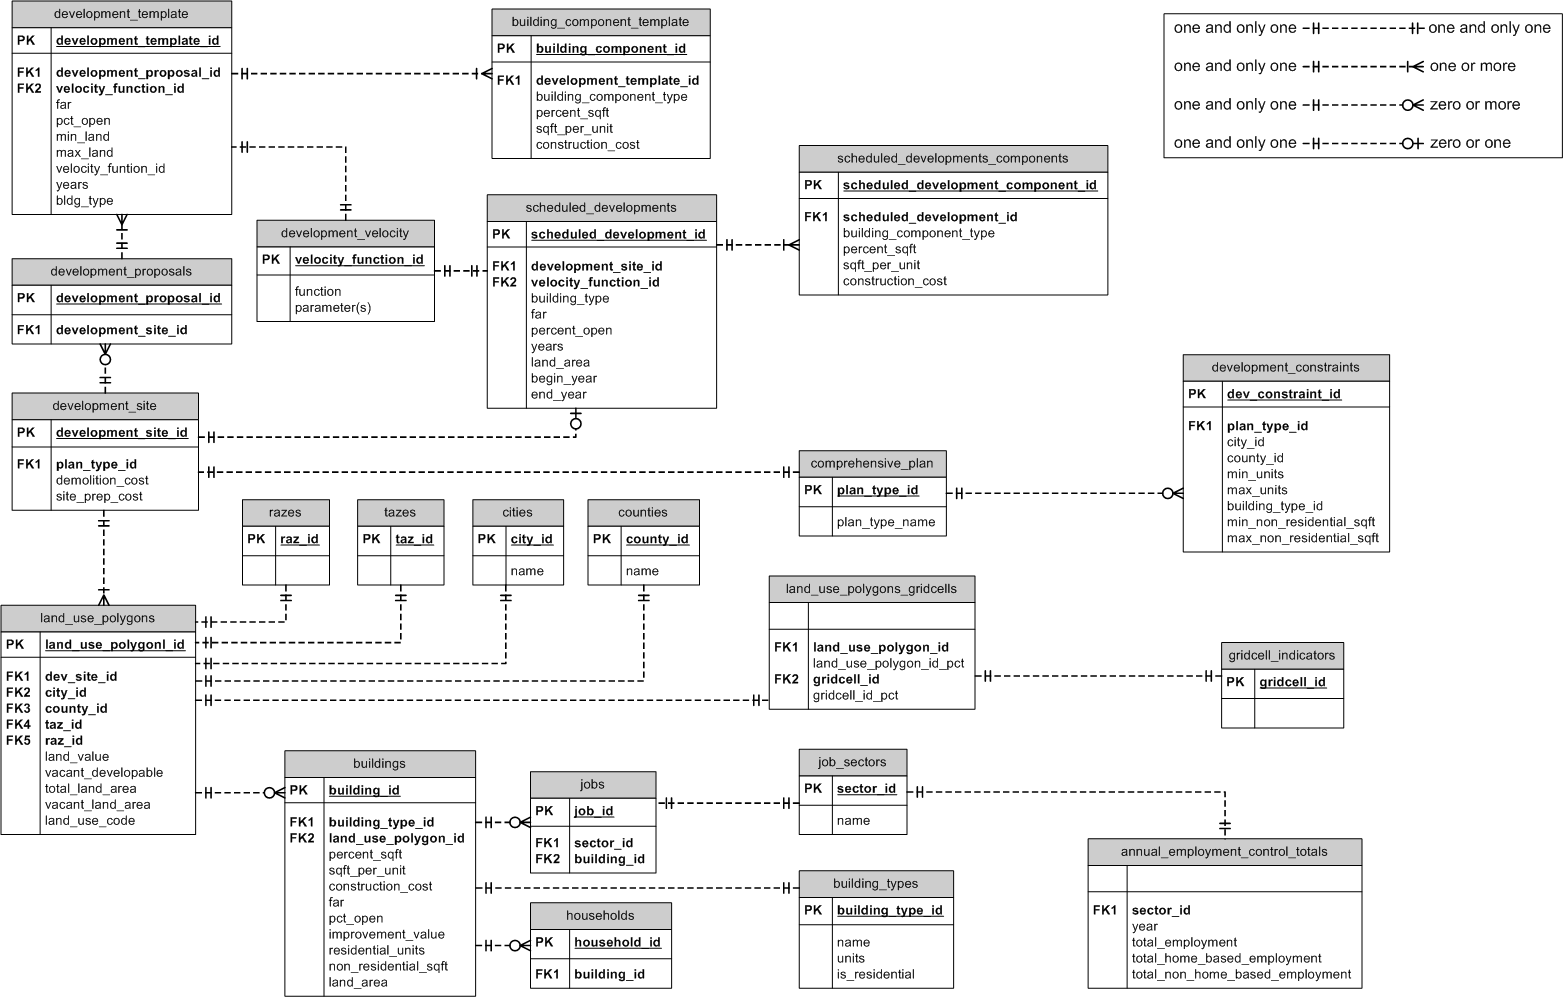
\includegraphics[scale=0.4]{../../datamodel/AZ-SMART_data_model_diagram_lupoly_based.png}
\caption{AZ-SMART Data Model Using Land Use Polygons}
\label{figLUPolyDataModel}
\end{center}
\end{sidewaysfigure}
\clearpage

\subsubsection{AZ-SMART Data Model Using Parcels}

Once the model system is created and tested using land use polygons, and for those counties that have
parcel data and for which AZ-SMART users prefer to do so, parcels could be substituted into the data model
in place of land use polygons.  This variant of the AZ-SMART data model is shown in Figure 
\ref{figParcelDataModel}.  Using parcel data provides more capacity to reflect spatial detail and information
in the assessor database, but conceptually and in terms of data model representation is almost identical to
the preceding data model based on land use polygons.

We recommend exploring the potential to transition to parcel-level in Maricopa and Pima County once the model
system is operational at a land use polygon level.  Since the data model was designed with this potential in mind,
the data structures allow easy substitution of parcels, without significantly affecting models and other code. 

The main difference between the land use polygon and parcel versions of the data model is that the source of
data would be quite different, and the parcel data could require additional tools for data checking and validation.

\begin{sidewaysfigure}[h]
\begin{center}
%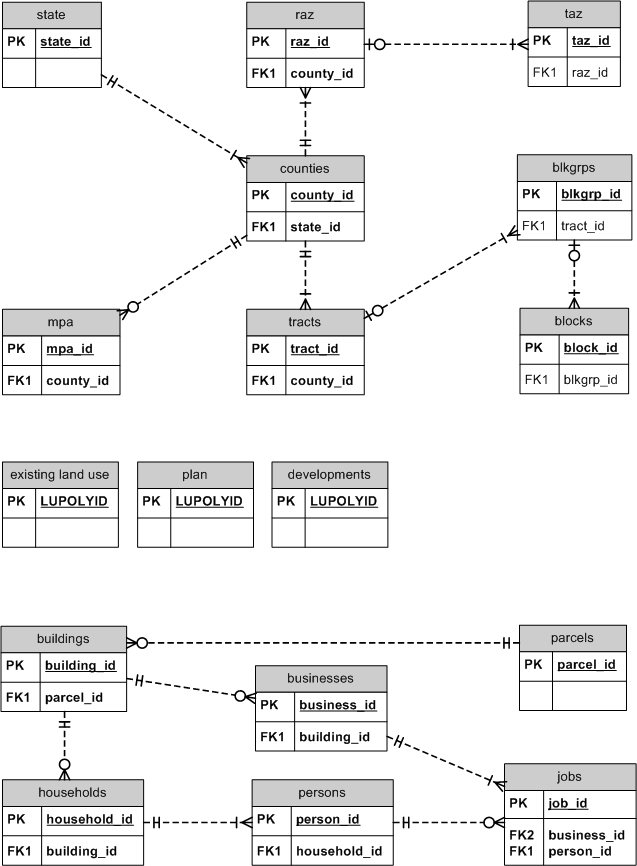
\includegraphics[scale=0.5]{figures/AZ-SMART_data_model_diagram.png}
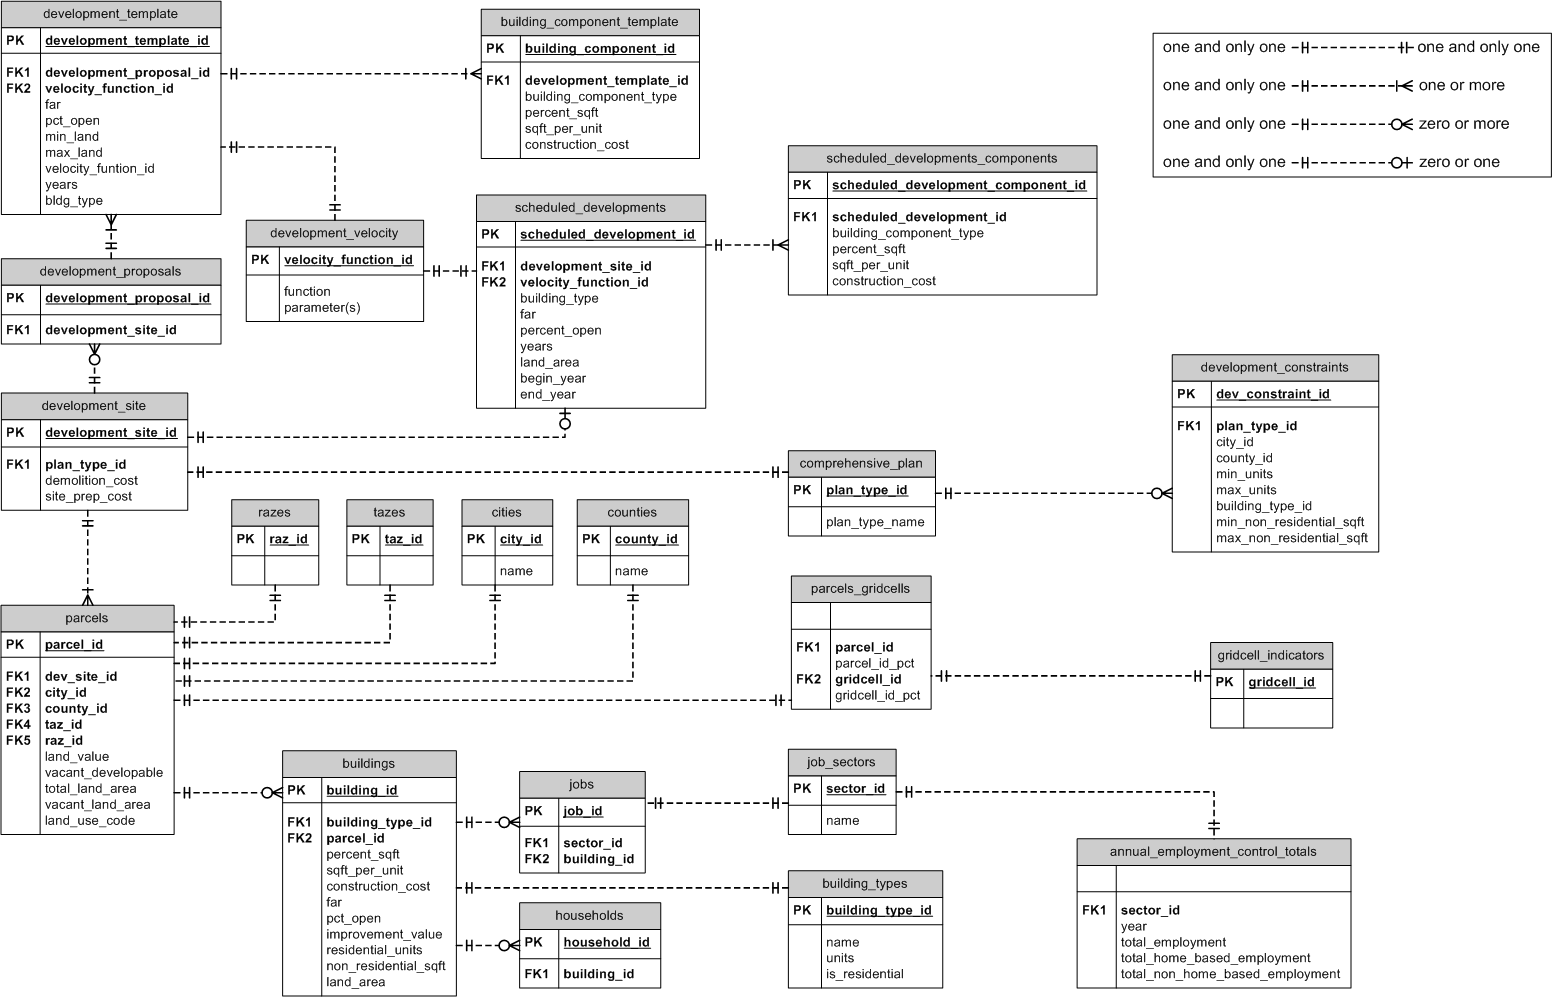
\includegraphics[scale=0.4]{../../datamodel/AZ-SMART_data_model_diagram_parcel_based.png}
\caption{AZ-SMART Data Model Using Parcels}
\label{figParcelDataModel}
\end{center}
\end{sidewaysfigure}
\clearpage
